\subsection{BÀI TẬP TRẮC NGHIỆM}

\ind{PHẦN I.} \inden{Câu trắc nghiệm nhiều phương án lựa chọn. Mỗi câu hỏi học sinh chỉ chọn một phương án.}\\
\setcounter{ex}{0}
\Opensolutionfile{ans}[ans/0H4-B2-1]
\begin{ex}%[0H1Y2-2]
	Cho tam giác $ABC$. Khẳng định nào sau đây đúng?
	\choice
	{$\overrightarrow{CA}+\overrightarrow{AB}=\overrightarrow{BC}$}
	{\True $\overrightarrow{AB}-\overrightarrow{AC}=\overrightarrow{CB}$}
	{$\overrightarrow{AA}+\overrightarrow{BB}=\overrightarrow{AB}$}
	{$\overrightarrow{AB}-\overrightarrow{AC}=\overrightarrow{BC}$}
	\loigiai{
		Ta có  $\overrightarrow{AB}-\overrightarrow{AC}=\overrightarrow{CB}$.}
\end{ex}

\begin{ex}%[0H1Y2-2]
	Cho hai điểm $A$ và $B$ phân biệt. Điều kiện cần và đủ để $I$ là trung điểm của đoạn thẳng $AB$ là
	\choice
	{$\overrightarrow{AI}=\overrightarrow{BI}$}
	{$\overrightarrow{IA}=\overrightarrow{IB}$}
	{$IA=IB$}
	{\True $\overrightarrow{IA}+\overrightarrow{IB}=\overrightarrow{0}$}
	\loigiai{
		Điều kiện cần và đủ để $I$ là trung điểm của đoạn $AB$ là$\overrightarrow{IA}+\overrightarrow{IB}=\overrightarrow{0}$.
	}
\end{ex}

\begin{ex}%[0H1B2-2]
	Cho ba điểm  $A$, $B$, $C$ phân biệt. Đẳng thức nào sau đây \textbf{sai}?
	\choice
	{
		$\overrightarrow{AB} + \overrightarrow{BC}=- \overrightarrow{CA}$
	}
	{
		$\overrightarrow{BC} = \overrightarrow{AC}+\overrightarrow{BA}$}
	{
		$\overrightarrow{CA} = \overrightarrow{BA}-\overrightarrow{BC}$}
	{
		\True $\overrightarrow{AB} = \overrightarrow{AC}-\overrightarrow{CB}$}
	\loigiai{
		Với ba điểm $A$, $B$, $C$ bất kỳ ta luôn có
		\begin{itemize}
			\item $\overrightarrow{CA} = \overrightarrow{BA}-\overrightarrow{BC}$ luôn đúng.
			\item $\overrightarrow{AC}+\overrightarrow{BA}=\overrightarrow{BA}+\overrightarrow{AC}=\overrightarrow{BC}$ luôn đúng.
			\item $\overrightarrow{AB} + \overrightarrow{BC}=\overrightarrow{AC}=-\overrightarrow{CA}$ luôn đúng.
			\item $\overrightarrow{AB} = \overrightarrow{AC}-\overrightarrow{CB}\Leftrightarrow \overrightarrow{AB} - \overrightarrow{AC}=-\overrightarrow{CB}\Leftrightarrow \overrightarrow{CB}=-\overrightarrow{CB}$ chỉ đúng khi $C\equiv B$.
		\end{itemize}
	}
\end{ex}

\begin{ex}%[0H1Y2-1]
	Cho 4 điểm $A, B, C, O$ phân biệt. Đẳng thức nào sau đây đúng?
	\choice
	{$\overrightarrow{AB}=\overrightarrow{OB}+\overrightarrow{OA}$}
	{$\overrightarrow{AB}=\overrightarrow{AC}+\overrightarrow{BC}$}
	{\True $\overrightarrow{OA}=\overrightarrow{CA}-\overrightarrow{CO}$}
	{$\overrightarrow{OA}=\overrightarrow{OB}-\overrightarrow{BA}$}
	\loigiai{
		Theo quy tắc trừ, ta có $\overrightarrow{O A}=\overrightarrow{C A}-\overrightarrow{C O}$.}
	
\end{ex}

\begin{ex}%[0H1B2-3]
	Cho vectơ $\overrightarrow{a}$ và $\overrightarrow{b}$ thỏa mãn $\overrightarrow{a}+\overrightarrow{b}=\overrightarrow{0}$. Với điểm $O$ bất kỳ, dựng vectơ $\overrightarrow{OA}=\overrightarrow{a},\overrightarrow{OB}=\overrightarrow{b}$. Chọn mệnh đề đúng.
	\choice
	{$A$ là trung điểm đoạn $OB$}
	{$\overrightarrow{OA}=\overrightarrow{OB}$}
	{$B$ là trung điểm đoạn $OA$}
	{\True $O$ là trung điểm đoạn $AB$}
	\loigiai{
		\immini
		{
			Ta có $\overrightarrow{a}+\overrightarrow{b}=\overrightarrow{0}\Leftrightarrow \overrightarrow{OA}+\overrightarrow{OB}=\overrightarrow{0}\Leftrightarrow \overrightarrow{OA}=-\overrightarrow{OB}=\overrightarrow{BO}$.\\
			Hay $O$ là trung điểm của $AB$. (như hình vẽ)
		}
		{
			\begin{tikzpicture}[scale=1, line join=round, line cap=round]
				\tkzDefPoints{0/0/O,-3/0/A}
				\tkzDefPointBy[translation = from A to O](O)    \tkzGetPoint{B}
				\draw[->] (O)--(A);
				\draw[->] (O)--(B);
				\tkzLabelPoints[below](A,B,O)
				\tkzDrawPoints[fill=black](O)
				\tkzMarkSegments[mark=x](O,A O,B)
			\end{tikzpicture}
		}
	}
\end{ex}

\begin{ex}
	Cho tứ giác ${ABCD}$. Tìm khẳng định đúng 
	\choice
	{ $\overrightarrow{AB}-\overrightarrow{AD}=\overrightarrow{CD}+\overrightarrow{BC}$ }
	{ \True $\overrightarrow{AB}-\overrightarrow{AC}=\overrightarrow{DB}-\overrightarrow{DC}$ }
	{ $\overrightarrow{BC}+\overrightarrow{AB}=\overrightarrow{DA}-\overrightarrow{DC}$ }
	{ $\overrightarrow{AC}-\overrightarrow{AD}=\overrightarrow{BD}-\overrightarrow{BC}$ }
	\loigiai{ 
		$\overrightarrow{AB}-\overrightarrow{AC}=\overrightarrow{DB}-\overrightarrow{DC}=\overrightarrow{CB}$. 
}\end{ex}

\begin{ex}%[0H1Y2-1]
	\immini[thm]{Cho $O$ là tâm của hình bình hành $ABCD$. Hỏi vectơ $\overrightarrow{AO}-\overrightarrow{DO}$ bằng vectơ nào dưới đây?
		\choice
		{$\overrightarrow{DC}$}
		{$\overrightarrow{BA}$}
		{\True $\overrightarrow{BC}$}
		{$\overrightarrow{AC}$}
	}{
		\begin{tikzpicture}[scale=0.7, line join=round, line cap=round]
			\tkzDefPoints{0/0/A,4/0/B,5/2/C}
			\tkzDefPointBy[translation=from B to C](A)\tkzGetPoint{D}
			\tkzInterLL(A,C)(B,D)\tkzGetPoint{O}
			\tkzDrawSegments(A,B B,C C,D D,A A,C B,D)
			\tkzDrawPoints[size=2,fill=black](A,B,C,D,O)
			\tkzLabelPoints[below,font=\footnotesize](A, B, O)
			\tkzLabelPoints[above,font=\footnotesize](C,D)
	\end{tikzpicture}}
	\loigiai{
		Ta có $\overrightarrow{AO}-\overrightarrow{DO}=\overrightarrow{AO}+\overrightarrow{OD}=\overrightarrow{AD}=\overrightarrow{BC}$.
	}
\end{ex}

\begin{ex}%[0H1B2-1]
	\immini[thm]{Cho hình bình hành $ABCD$ tâm $O$. Đẳng thức nào sau đây đúng?
		\choice
		{\True $\overrightarrow{OA}+\overrightarrow{OC}=\overrightarrow{0}$}
		{$\overrightarrow{OA}-\overrightarrow{OC}=\overrightarrow{0}$}
		{$\overrightarrow{OA}+\overrightarrow{CO}=\overrightarrow{0}$}
		{$\overrightarrow{AO}+\overrightarrow{OC}=\overrightarrow{0}$}
	}{
		\begin{tikzpicture}[scale=0.7, line join=round, line cap=round]
			\tkzDefPoints{0/0/A,4/0/B,5/2/C}
			\tkzDefPointBy[translation=from B to C](A)\tkzGetPoint{D}
			\tkzInterLL(A,C)(B,D)\tkzGetPoint{O}
			\tkzDrawSegments(A,B B,C C,D D,A A,C B,D)
			\tkzDrawPoints[size=2,fill=black](A,B,C,D,O)
			\tkzLabelPoints[below,font=\footnotesize](A, B, O)
			\tkzLabelPoints[above,font=\footnotesize](C,D)
	\end{tikzpicture}}
	\loigiai{
		Ta có $ABCD$ là hình bình hành nên $O$ là trung điểm của $AC$.\\
		Vậy $\overrightarrow{OA}+\overrightarrow{OC}=\overrightarrow{0}$.
	}
	%<MyLT>
\end{ex}

\begin{ex}
	\immini[thm]{Cho lục giác đều $ABCDEF$ tâm $O$. Khẳng định nào sau đây là sai?
		\haicot
		{$\overrightarrow{O A}+\overrightarrow{O C}-\overrightarrow{E O}=\overrightarrow{0}$}
		{$\overrightarrow{B C}-\overrightarrow{E F}=\overrightarrow{A D}$}
		{$\overrightarrow{O A}-\overrightarrow{O E}=\overrightarrow{E B}-\overrightarrow{O C}$}
		{\True $\overrightarrow{A B}+\overrightarrow{C D}-\overrightarrow{E F}=\overrightarrow{0}$}
	}
	{
		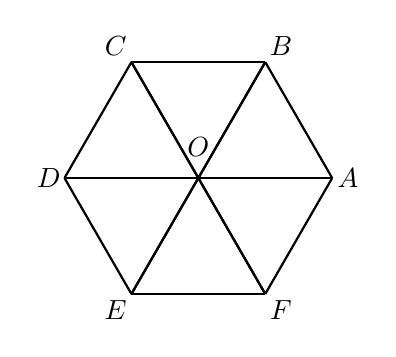
\begin{tikzpicture}[scale=1.7,thick]
			\foreach \x in {0,60,...,300} {
				\draw (\x:1 cm) -- (\x + 60:1 cm);
				\draw (\x:1 cm) -- (\x + 180:1 cm);
			}
			\draw  (0:1 cm) node[shift={(0.2,0)}] {$A$}; \draw  (60:1 cm) node[shift={(0.2,0.2)}] {$B$};
			\draw  (120:1 cm) node[shift={(-0.2,0.2)}] {$C$}; \draw  (180:1 cm) node[shift={(-0.2,0)}] {$D$};
			\draw  (240:1 cm) node[shift={(-0.2,-0.2)}] {$E$}; \draw  (300:1 cm) node[shift={(0.2,-0.2)}] {$F$};
			\draw  (0,0.08 ) node[above] {$O$};
		\end{tikzpicture}
	}
	\loigiai{
		Ta có: $\overrightarrow{A B}+\overrightarrow{C D}-\overrightarrow{E F}=\overrightarrow{A B}+\overrightarrow{B O}-\overrightarrow{O A}=\overrightarrow{A O}-\overrightarrow{O A}=2 \overrightarrow{A O} \neq \overrightarrow{0}$.
	}
\end{ex}

\begin{ex}%[WTT-1234 câu TN10, Phan Minh Tâm]%[0H1B2-4]%
	Cho tam giác $ABC$. Vị trí của điểm $M$ sao cho $\overrightarrow{MA}-\overrightarrow{MB}+\overrightarrow{MC}=\overrightarrow{0}$ là
	\choice
	{$M$ trùng $C$}
	{\True $M$ là đỉnh thứ tư của hình bình hành $CABM$}
	{$M$ là đỉnh thứ tư của hình bình hành $CBAM$}
	{$M$ trùng $B$}
	\loigiai{
		$\overrightarrow{MA}-\overrightarrow{MB}+\overrightarrow{MC}=\overrightarrow{0} \Leftrightarrow \overrightarrow{BA}+\overrightarrow{MC}=\overrightarrow{0} \Leftrightarrow \overrightarrow{CM}=\overrightarrow{BA}$.\\
		Vậy $M$ thỏa mãn $CBAM$ là hình bình hành.}
\end{ex}

\begin{ex}%[0H1B2-5]
	Cho hình vuông $ABCD$ cạnh $a$, tâm $O$. Tính độ dài của vectơ $\overrightarrow{OA}+\overrightarrow{OB}$.
	\choice
	{\True $a$}
	{$2a$}
	{$\dfrac{a}{2}$}
	{$3a$}
	\loigiai{
		$\left|\overrightarrow{OA}+\overrightarrow{OB}\right|=\left|\overrightarrow{CO}+\overrightarrow{OB}\right|=\left|\overrightarrow{CB}\right|=CB=a$.}
\end{ex}

\begin{ex}%[0H1B2-5]
	Cho hình chữ nhật $ABCD$ có $AB=4a$ và $AD=3a$. Độ dài của vectơ $\overrightarrow{BA}+\overrightarrow{DA}$ bằng
	\choice
	{$7a$}
	{$6a$}
	{\True $5a$}
	{$2a\sqrt{3}$}
	\loigiai{
		\immini{Áp dụng quy tắc hình hình hành ta có
			\begin{eqnarray*}
				&&\overrightarrow{AB}+\overrightarrow{AD}=\overrightarrow{AC}\Rightarrow\overrightarrow{BA}+\overrightarrow{DA}=\overrightarrow{CA}.\\
				&\Rightarrow&\left|\overrightarrow{BA}+\overrightarrow{DA}\right|=\left|\overrightarrow{CA}\right|=AC=\sqrt{AB^2+AD^2}=5a.
			\end{eqnarray*}
		}
		{\begin{tikzpicture}[scale=0.6, font=\footnotesize, line join=round, line cap=round, >=stealth]
				\tkzDefPoints{0/0/A,4/0/B,0/3/D,4/3/C}
				\tkzDrawSegments(A,B B,C C,D D,A)
				\tkzDrawPoints(A,B,C,D)
				\tkzLabelPoints[above left](D)
				\tkzLabelPoints[above right](C)
				\tkzLabelPoints[below left](A)
				\tkzLabelPoints[below right](B)
				\draw[->](A)--(B);
				\draw[->](A)--(D);
				\draw[->](A)--(C);
	\end{tikzpicture}}}
\end{ex}

\Closesolutionfile{ans}

\ind{PHẦN II.} \inden{Câu trắc nghiệm đúng sai. Trong mỗi ý a), b), c), d) ở mỗi câu, học sinh chọn đúng hoặc sai.}\\
\Opensolutionfile{ans}[ans/0H4-B2-2]

\begin{ex}%[0H5H2-2]%Câu 2
	Cho tam giác $ ABC$. Các điểm $M$, $N$, $P$ lần lượt là trung điểm của $ AB$, $AC$, $BC$. Xét tính đúng sai của các khẳng định sau:
	\choiceTF
	{\True $\overrightarrow{AM}-\overrightarrow{AN}=\overrightarrow{NM}$}
	{$\overrightarrow{MN}-\overrightarrow{NC}=\overrightarrow{MP}$}
	{\True $\overrightarrow{MN}-\overrightarrow{PN}=\overrightarrow{MP}$}
	{\True $\overrightarrow{PB}+\overrightarrow{CP}=\overrightarrow{CB}$}
	\loigiai{
		\begin{center}
			{\begin{tikzpicture}[scale=0.8, font=\footnotesize, line join=round, line cap=round, >=stealth]
					\def\a{3} \def\b{4}
					\path
					(0:0) coordinate (B)
					(0:\b) coordinate (C)
					(70:\a) coordinate (A)
					($(A)!1/2!(B)$) coordinate (M)
					($(A)!1/2!(C)$) coordinate (N)
					($(C)!1/2!(B)$) coordinate (P);
					\draw (A)--(B)--(C)--cycle (M)--(N)--(P)--cycle;
					\foreach \i/\g in {A/90, B/180, C/0, M/150,N/30,P/-90}{\filldraw[black](\i) circle (1pt) ($(\i)+(\g:3mm)$) node[scale=1]{$\i$};}
			\end{tikzpicture}}
		\end{center}
		\begin{itemchoice}
			\itemch Đúng, vì theo quy tắc hiệu, ta có $\overrightarrow{AM}-\overrightarrow{AN}=\overrightarrow{NM}$.
			\itemch Sai, vì $\overrightarrow{MN}-\overrightarrow{NC}=\overrightarrow{MN}-\overrightarrow{MP}=\overrightarrow{PN}$.
			\itemch  Đúng, vì $\overrightarrow{MN}-\overrightarrow{PN}=\overrightarrow{MN}+\overrightarrow{NP}=\overrightarrow{MP}$.
			\itemch Đúng, vì $\overrightarrow{PB}+\overrightarrow{CP}=\overrightarrow{CP}+\overrightarrow{PB}=\overrightarrow{CB}$.
		\end{itemchoice}
	}
\end{ex}

\begin{ex}%[0H5V2-4]%Câu 3
	Cho hình bình hành $ ABCD$, gọi $ O$ là giao điểm của $ AC$ và $ BD$. Gọi $ G$ là trọng tâm tam giác $ ABC$.  Xét tính đúng sai của các khẳng định sau:
	\choiceTF
	{\True $ \left| \overrightarrow{AB}+\overrightarrow{AD}\right|=\left| \overrightarrow{AC}\right|$}
	{$\overrightarrow{AB}+\overrightarrow{BD}=\overrightarrow{CB}$}
	{$\overrightarrow{OA}+\overrightarrow{OB}=\overrightarrow{OC}+\overrightarrow{OD}$}
	{\True $ 3\left|\overrightarrow{GD}+\overrightarrow{GB}\right|=2OD$}
	\loigiai{
		\begin{center}
			\begin{tikzpicture}[scale=0.8, font=\footnotesize, line join=round, line cap=round, >=stealth]
				\def\a{3} \def\b{4}
				\path
				(0:0) coordinate (A)
				(0:\b) coordinate (D)
				(50:\a) coordinate (B)++(0:\b) coordinate (C)
				($(C)!1/2!(A)$) coordinate (O)
				($(B)!2/3!(O)$) coordinate (G)
				($(D)!2/3!(O)$) coordinate (N);
				\draw (A)--(B)--(C)--(D)--cycle (A)--(C) (B)--(D);
				\foreach \i/\g in {A/-90, B/90, C/90, D/-90,O/-90,G/30,N/60}{\filldraw[black](\i) circle (1pt) ($(\i)+(\g:3mm)$) node[scale=1]{$\i$};}
			\end{tikzpicture}
		\end{center}
		\begin{itemchoice}
			\itemch Theo quy tắc hình bình hành thì $\overrightarrow{AB}+\overrightarrow{AD}=\overrightarrow{AC}$ nên $ \left| \overrightarrow{AB}+\overrightarrow{AD}\right| =\left|\overrightarrow{AC}\right|$. Vậy mệnh đề ĐÚNG.
			\itemch Ta có $\overrightarrow{AB}+\overrightarrow{BD}=\overrightarrow{AD}=-\overrightarrow{CB}.$ Vậy mệnh đề SAI.
			\itemch  Ta có $\overrightarrow{OA}+\overrightarrow{OB}+\overrightarrow{OC}+\overrightarrow{OD}=\overrightarrow 0\Leftrightarrow\overrightarrow{OA}+\overrightarrow{OB}=-\left(\overrightarrow{OC}+\overrightarrow{OD}\right)$. Vậy mệnh đề SAI.
			\itemch Gọi $N$ là trọng tâm tam giác $ ADC$. Khi đó $ DN=NG=GB=\dfrac{2}{3}OD$.\\
			Ta có $\overrightarrow{GD}+\overrightarrow{GB}=\overrightarrow{GN}+\overrightarrow{ND}+\overrightarrow{GB}=\overrightarrow{ND}$.\\
			Do đó $ 3\left|\overrightarrow{GD}+\overrightarrow{GB}\right|=3\left|\overrightarrow{ND}\right|=3ND=2OD$. Vậy mệnh đề ĐÚNG.
		\end{itemchoice}
	}
\end{ex}

\begin{ex}%[0H1K2-5]%
	Cho tam giác đều $ABC$ có cạnh bằng $a$ , trọng tâm $G$ . Gọi $M$, $I$ lần lượt là trung điểm của $BC$ và $AC$. Xét tính đúng sai của các khẳng định sau:
	\choiceTF
	{\True $\vec{GA}+\vec{GB}+\vec{GC}=\vec{0}$}
	{$\vec{AB}+\vec{AC}=\vec{AM}$}
	{$\left|\vec{AB}+\vec{BC}\right|=2a$}
	{\True $\left|\vec{AB}-\vec{GC}\right|=\dfrac{2a\sqrt 3}{3}$}
	\loigiai{
		\begin{center}
			\begin{tikzpicture}[>=stealth,line join=round,line cap=round,font=\footnotesize,scale=1]
				\tkzDefPoints{0/0/B, 5/0/C, 2.5/4/A}
				\coordinate (I) at ($(A)!0.5!(C)$);
				\coordinate (M) at ($(B)!0.5!(C)$);
				\tkzCentroid(A,B,C)\tkzGetPoint{G}
				\tkzDefPointBy[symmetry = center I](G) \tkzGetPoint{D}
				\tkzDrawPoints(A,B,C,I,G,D)
				\tkzLabelPoints[above](A,I)
				\tkzLabelPoints[left](G,B)
				\tkzLabelPoints[right](C,D)
				\tkzLabelPoints[below](M)
				\tkzDrawSegments(A,B B,C A,C A,M G,C A,D D,C B,D)
			\end{tikzpicture}
		\end{center}
	\begin{itemchoice}
		\itemch Theo tính chất trọng tâm thì $\vec{GA}+\vec{GB}+\vec{GC}=\vec{0}$.
		\itemch Gọi $E$ là điểm đối xứng của $G$ qua $M$. Suy ra $\vec{AB}+\vec{AC}=\vec{AE}$.
		\itemch Ta có $\left|\vec{AB}+\vec{BC}\right|=\left|\vec{AC}\right|=AC=a$.
		\itemch Gọi $D$ là điểm đối xứng với $G$ qua $I$. Khi đó tứ giác $AGCD$ là hình bình hành. Suy ra $\vv{GC}=\vv{AD}$.\\
		$\vv{AB}-\vv{GC}=\vv{AB}-\vv{AD}=\vv{DB}\Rightarrow\left|\vv{AB}-\vv{GC}\right|=DB=2BG=\dfrac{4}{3}BI=\dfrac{2a\sqrt 3}{3}$.
	\end{itemchoice}
	}
\end{ex}

\begin{ex}%[0H5V2-6]%Câu 4
	Cho ba lực $\overrightarrow{MA}=\overrightarrow{F_1}$, $\overrightarrow{MB}=\overrightarrow{F_2}$, và $\overrightarrow{MC}=\overrightarrow{F_3}$ cùng tác động vào một vật tại điểm $M$ và vật đứng yên. Cho biết cường độ của $\overrightarrow{F}_1$, $\overrightarrow{F}_2$ đều là $100$N và $\widehat{AMB}=60^\circ$.  Xét tính đúng sai của các khẳng định sau:
	\choiceTF
	{\True Lực tổng hợp tác dụng lên vật có độ lớn bằng $0$ N}
	{\True $\widehat{AMC}=150^\circ$}
	{\True Cường độ của lực $\overrightarrow{F}_3$ là $100\sqrt 3$ N}
	{Khi $\widehat{AMB}=90^\circ$ thì cường độ của lực $\overrightarrow{F}_3$ là  $100$ N}
	\loigiai{
		\begin{center}
			\begin{tikzpicture}[scale=1, font=\footnotesize, line join=round, line cap=round, >=stealth]
				\def\a{2} \def\b{3.2}
				\path
				(30:\a) coordinate (A)
				(-30:\a) coordinate (B)
				(-180:\b) coordinate (C)
				(0:0) coordinate (M)
				($(A)!1/2!(B)$) coordinate (N)
				($(M)!2!(N)$) coordinate (P);
				\draw[->] (M)--(A) node[midway,above] {$\overrightarrow{F}_1$};
				\draw[->] (M)--(B)node[midway,below] {$\overrightarrow{F}_2$};
				\draw[->] (M)--(C)node[midway,above] {$\overrightarrow{F}_3$};
				\draw[dashed,->] (M)--(P);
				\draw[dashed] (A)--(B) (A)--(P)--(B);
				\pic [draw, angle eccentricity=1.7] {angle = B--M--A};
				\foreach \i/\g in {A/90, B/-90, C/90, M/-90,N/-50,P/0}{\filldraw[black](\i) circle (1pt) ($(\i)+(\g:3mm)$) node[scale=1]{$\i$};}
			\end{tikzpicture}
		\end{center}
		\begin{itemchoice}
			\itemch Vì vật đứng yên nên $\overrightarrow{F_1}+\overrightarrow{F_2}+\overrightarrow{F_3}=\overrightarrow 0$. Hay lực tổng hợp tác dụng lên vật có độ lớn bằng $0$ N.
			\itemch Gọi $N$ là trung điểm $AB$, và $P$ là điểm đối xứng với $M$ qua $N$, khi đó tứ giác $MAPB$ là hình thoi với tâm là điểm $N$  và $MP$ là phân giác góc $\widehat{AMB}$.\\
			Ta có $\widehat{AMC}=180^\circ-\widehat{AMN}=180^\circ-30^\circ=150^\circ$.
			\itemch Vật đứng yên nên
			\begin{eqnarray*}
				&&\overrightarrow{F}+\overrightarrow{F}_2+\overrightarrow{F}_3=\overrightarrow 0\\
				&\Leftrightarrow&\overrightarrow{MA}+\overrightarrow{MB}+\overrightarrow{MC}=\overrightarrow 0\\
				&\Leftrightarrow&\overrightarrow{MC}=-\left(\overrightarrow{MA}+\overrightarrow{MB}\right)=-\overrightarrow{MP}.
			\end{eqnarray*}
			Ta có tam giác $MAB$ đều và $MN=\dfrac{100\sqrt 3}{2}=50\sqrt 3 $ nên  
			$$MC=MP=2MN=2\cdot 50\sqrt 3=100\sqrt 3.$$
			\itemch Khi $\widehat{AMB}=90^\circ$ thì $MP=MA\sqrt{2}=100\sqrt{2}$.\\
			Do đó cường độ của lực $\overrightarrow{F}_3$ là  $100\sqrt{2}$ N.
		\end{itemchoice}
	}
\end{ex}

\Closesolutionfile{ans}

\ind{PHẦN III.} \inden{Câu trắc nghiệm trả lời ngắn.}\\
\Opensolutionfile{ans}[ans/0H4-B2-3]

\begin{ex}%[Phạm Tuấn]%[941-960-YouTuTu]%[0H1K2-5]%
	Cho ba vectơ $\vec{u}$, $\vec{v}$ và $\vec{w}$ như hình vẽ. Biết mỗi ô vuông có
	kích thước $1\mathrm{cm} \times 1\mathrm{cm}$, tính độ  dài của vectơ
	$\vec{a} = \vec{u} + \vec{v} + \vec{w}$ (kết quả tính theo đơn vị cm và làm tròn đến 2 chữ số thập phân).\\
	\shortans[oly]{$3,16$}
	\begin{center}
		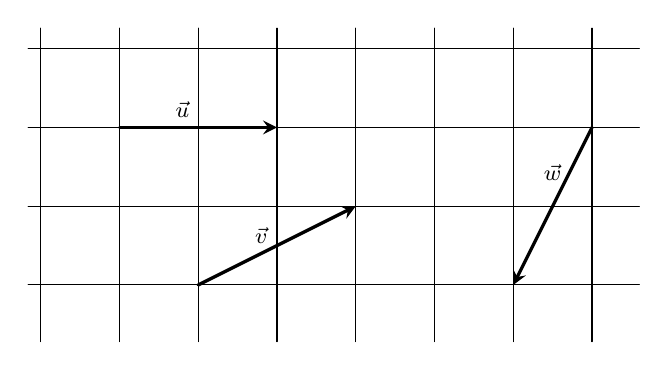
\begin{tikzpicture}[>=stealth,line join=round,line cap=round,font=\footnotesize,scale=1]
			\draw [xstep=1cm,ystep=1cm] (-0.16,-1.72) grid (7.6,2.26);
			\coordinate (A) at (1,1); \coordinate (B) at (3,1);
			\coordinate (C) at (2,-1); \coordinate (D) at (4,0);
			\coordinate (E) at (7,1); \coordinate (F) at (6,-1);
			\draw[->,very thick] (A)--(B); \draw (1.8,1) node[above] {$\vec{u}$} ;
			\draw[->,very thick] (C)--(D); \draw (2.8,-0.6) node[above] {$\vec{v}$} ;
			\draw[->,very thick] (E)--(F); \draw (6.5,0.2) node[above] {$\vec{w}$} ;
		\end{tikzpicture}
	\end{center}
	\loigiai{
		\begin{center}
			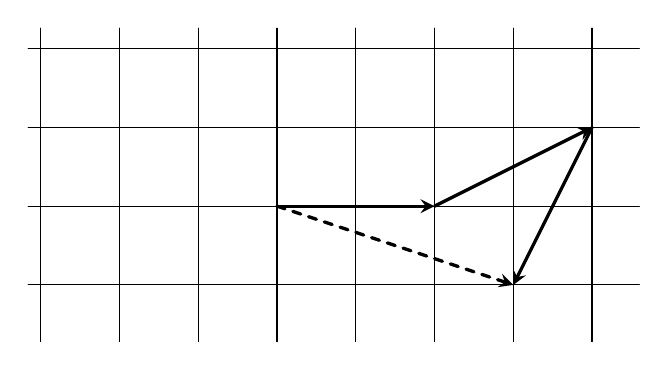
\begin{tikzpicture}[>=stealth,line join=round,line cap=round,font=\footnotesize,scale=1]
				\draw [xstep=1cm,ystep=1cm] (-0.16,-1.72) grid (7.6,2.26);
				%\coordinate (A) at (1,1); \coordinate (B) at (3,1);
				%\coordinate (C) at (2,-1); \coordinate (D) at (4,0);
				\coordinate (E) at (7,1); \coordinate (F) at (6,-1);
				\coordinate (G) at (5,0); \coordinate (I) at (3,0);
				% \draw[->,very thick,dashed] (A)--(B); \draw (1.8,1) node[above] {$\vec{u}$} ;
				%\draw[->,very thick] (C)--(D); \draw (2.8,-0.6) node[above] {$\vec{v}$} ;
				\draw[->,very thick] (E)--(F);
				\draw[->,very thick] (G)--(E);
				\draw[->,very thick] (I)--(G);
				\draw[->,very thick,dashed] (I)--(F);
				\tkzLabelPoints[above](I,G,E)
				\tkzLabelPoints[below](F)
			\end{tikzpicture}
		\end{center}
		Dựng $\vec{IG}=\vec{u}$, $\vec{GE}=\vec{v}$, $\vec{EF}=\vec{w}$ như hình vẽ.\\
		Khi đó, $\vec{a} = \vec{u} + \vec{v} + \vec{w}=\vec{IF}.$ Suy ra $\left|\vec{a}\right|=IF=\sqrt{10}\approx3,16$ cm.
	}
\end{ex}

\begin{ex}
	Cho $\triangle ABC$ vuông tại $A$ có $AB=AC=2$ cm. Tính $\left|\overrightarrow{AB}+\overrightarrow{AC}\right|$ (kết quả tính theo đơn vị cm và làm tròn đến 2 chữ số thập phân).\\
	\shortans[oly]{$2,83$}
	\loigiai{
		\immini{Ta có $\overrightarrow{AB} + \overrightarrow{AC} = \overrightarrow{AD}$. Khi đó $\left|\overrightarrow{AB}+\overrightarrow{AC}\right| = \left|\overrightarrow{AD}\right| = AD$.\\
			Theo định lý Py-ta-go ta có $AD = \sqrt{AB^2+AC^2} = 2\sqrt{2} \approx 2,83$.}{
			\begin{tikzpicture}
				\tkzDefPoints{0/3/B,0/0/A,3/0/C,3/3/D}
				\tkzLabelPoints[above left](B)
				\tkzLabelPoints[above right](D)
				\tkzLabelPoints[below left](A)
				\tkzLabelPoints[below right](C)
				\tkzDrawPoints(A,B,C)
				\tkzDrawSegments(B,C B,D C,D)
				\tkzDrawVectors(A,B A,C A,D)
		\end{tikzpicture}}
	}
\end{ex}

\begin{ex}
	\immini[thm]{Cho ba lực $\vec{F}_1=\overrightarrow{M A}$, $\overrightarrow{F_2}=\overrightarrow{M B}$, $\overrightarrow{F_3}=\overrightarrow{M C}$ cùng tác động vào một vật tại điểm $M$ và vật đứng yên như hình vẽ. Biết cường độ của lực $\vec{F}_1$ là $50 N$, $\widehat{A M B}=120^{\circ}$, $\widehat{A M C}=150^{\circ}$. Cường độ của lực $\vec{F}_3$ bằng bao nhiêu? (kết quả tính bằng đơn vị N làm tròn đến 1 chữ số thập phân)\\
	\shortans[oly]{$43,3$}}{
\begin{tikzpicture}[smooth,font=\footnotesize,scale=0.8,>=Latex]
	\path
	(0,0) coordinate (M)
	(3,0) coordinate (M1)
	(-5,0) coordinate (A)
	($(M)!1!60:(M1)$) coordinate (B)
	($(M)!1.3!-30:(M1)$) coordinate (C)
	;
	\fill[ball color=red](0,0) circle (0.16);
	\draw[->] (M)--(A);
	\draw[->] (M)--(B);
	\draw[->] (M)--(C);
	\foreach \x/\g in {A/180,B/0,C/0,M/0} \draw [fill=black] (\x) circle (.05) + (\g:.5) node{$\x$};
	\begin{scope}
		\clip (B)--(M)--(A);
		\draw[double] (M) circle(0.6cm);
	\end{scope}
	\begin{scope}
	\clip (C)--(M)--(A);
	\draw (M) circle(0.4cm);
	\end{scope}
	\node[above] at (-0.4,0.5) {$120^\circ$};
	\node[below] at (0,-0.4) {$150^\circ$};
\end{tikzpicture}}
\loigiai{
Ta có $\widehat{A M B}=120^{\circ}, \widehat{A M C}=150^{\circ} \Rightarrow \widehat{B M C}=360^{\circ}-120^{\circ}-150^{\circ}=90^{\circ}$.\\
Vẽ hình chữ nhật $M C D B$, có $\widehat{C M D}=180^{\circ}-\widehat{A M C}=180^{\circ}-150^{\circ}=30^{\circ}$.
\begin{center}
	\begin{tikzpicture}[smooth,font=\footnotesize,scale=0.8,>=Latex]
		\path
		(0,0) coordinate (M)
		(-5,0) coordinate (A)
		(5,0) coordinate (D)
		(1.25,2.17) coordinate (B)
		(3.75,-2.17) coordinate (C)
		;
		\fill[ball color=red](0,0) circle (0.16);
		\draw[->] (M)--(A);
		\draw[->] (M)--(B);
		\draw[->] (M)--(C);
		\draw[->] (M)--(D);
		\draw (C)--(D)--(B);
		\foreach \x/\g in {A/180,B/0,C/0,M/0,D/0} \draw [fill=black] (\x) circle (.05) + (\g:.5) node{$\x$};
		\begin{scope}
			\clip (B)--(M)--(A);
			\draw[double] (M) circle(0.6cm);
		\end{scope}
		\begin{scope}
			\clip (C)--(M)--(A);
			\draw (M) circle(0.4cm);
		\end{scope}
		\node[above] at (-0.4,0.5) {$120^\circ$};
		\node[below] at (0,-0.4) {$150^\circ$};
	\end{tikzpicture}
\end{center}
Vì vật đứng yên nên tổng hợp lực tác động vào vật bằng $0 \Rightarrow M D=M A=50$.

$$
\cos \widehat{C M D}=\frac{M C}{M D} \Rightarrow M C=M D \cdot \cos 30^{\circ}=50 \cdot \frac{\sqrt{3}}{2}=25 \sqrt{3}
$$


Vậy $\left|\vec{F}_3\right|=F_3=M C=25 \sqrt{3} N \approx 43,3$ N.
}
\end{ex}

\begin{ex}%[0H1B2-5]
	\immini[thm]{Người ta thiết kế một bến phà như hình vẽ bên. Khi phà di chuyển từ bờ $M$ sang bờ $N$ với vận tốc $v_1=10$ m/s theo hướng vuông góc với bờ, do nước chảy với vận tốc $v_2=6 $ m/s cùng phương với bờ nên phà sẽ đi theo hướng của vectơ $\overrightarrow{v}$ là vectơ tổng của hai vectơ $\overrightarrow{v}_1$ và $\overrightarrow{v}_2$. Hãy tính vận tốc $v$ (m/s) của phà khi đi từ bờ $M$ sang bờ $N$ (kết quả làm tròn đến 1 chữ số thập phân).\\
		\shortans[oly]{$11,7$}
	}{
		\begin{tikzpicture}[scale=0.7,line join=round, line cap=round,>=stealth,transform shape]
			\tkzDefPoints{0/0/M, 0.6/0/A, 0.5/0.3/B, 2.2/0/C, 2.6/0.5/E, 4/0/V1, 0/-1/ttv2, 0/-3/M', 6/0/N'}
			\tkzDefPointBy[translation=from A to C](B)\tkzGetPoint{D}
			\tkzDefPointBy[translation=from M to M'](N')\tkzGetPoint{N}
			\tkzDefPointBy[translation=from M to ttv2](C)\tkzGetPoint{V2}
			\tkzDefPointBy[translation=from A to C](V2)\tkzGetPoint{V}
			\draw[->] (C)--(V1);
			\draw[->] (C)--(V2);
			\draw[->] (C)--(V);
			\tkzDrawLine[add=0.5 and 0.5](M,M')
			\tkzDrawLine[add=0.5 and 0.5](N,N')
			\tkzDrawSegments(A,B A,C C,E B,D E,D)
			\tkzDrawPoints[fill=black](M,N)
			\node[right] at (V1){$\overrightarrow{v}_1$};
			\node[below] at (V2){$\overrightarrow{v}_2$};
			\node[right] at (V){$\overrightarrow{v}$};
			\tkzLabelPoints[left](M,N)
		\end{tikzpicture}
	}
	\loigiai{
		Ta có $\overrightarrow{v}=\overrightarrow{v}_1+\overrightarrow{v}_2$. Theo quy tắc hình bình hành ta có $\left|\overrightarrow{v}\right|=\left|\overrightarrow{v}_1+\overrightarrow{v}_2\right|=\sqrt{v_1^2+v_2^2}=\sqrt{36+100}$. \\
		Suy ra thuyền chạy với vận tốc $\left|\overrightarrow{v}\right|=\sqrt{136}=2\sqrt{34} \approx 11,7$ m/s.}
\end{ex}


\Closesolutionfile{ans}